% AVD612 LMS presentation, editable Beamer source.
% Replace names/institute, verify figures, and practice for 10 minutes.
\documentclass[aspectratio=169,11pt]{beamer}
\usetheme{Boadilla}
\usecolortheme{default}
\usepackage{amsmath,amssymb,graphicx,booktabs,tikz}
\usetikzlibrary{arrows.meta,positioning}
\definecolor{navy}{HTML}{1F3557}
\definecolor{accent}{HTML}{146C9C}
\setbeamercolor{structure}{fg=navy}
\setbeamercolor{frametitle}{bg=navy,fg=white}
\setbeamercolor{title}{fg=navy}
\setbeamercolor{block title}{bg=navy!12,fg=navy}
\setbeamercolor{block body}{bg=navy!4,fg=black}
\setbeamertemplate{navigation symbols}{}
\setbeamertemplate{footline}[frame number]
\graphicspath{{../results/simulation_graphs/}}
\title[Training-Based LMS Equalizer]{Training-Based LMS Adaptive Equalizer}
\subtitle{BPSK and QPSK Communication Link Simulation}
\author{Member 1 \and Member 2 \and Member 3}
\institute{AVD612 Course Project \quad \textbullet\quad Institute / Department (replace)}
\date{Semester Project Presentation}
\begin{document}

\begin{frame}
\titlepage
\vfill
\centering{\scriptsize Three-member team \quad | \quad 10-minute presentation \quad | \quad Python simulation}
\end{frame}

\begin{frame}{1. What is an LMS equalizer?}
\begin{block}{Definition}
A linear finite-impulse-response (FIR) filter that \textbf{adaptively adjusts its coefficients} to recover symbols distorted by a channel with memory.
\end{block}
\medskip
\begin{itemize}\setlength{\itemsep}{9pt}
\item LMS = \textbf{Least Mean Squares}; it uses a known training sequence to reduce error.
\item Main problem: \textbf{inter-symbol interference (ISI)}.
\item Input: received BPSK or QPSK symbols; output: improved symbol estimates.
\item Objective: lower mean-square error, then compare bit-error rates on new test data.
\end{itemize}
\end{frame}

\begin{frame}{2. Why do communication links need equalizers?}
\begin{columns}[T]
\column{.57\textwidth}
\begin{block}{Simple channel model}
\[r[n]=0.90s[n]+0.65s[n-1]-0.35s[n-2]+v[n]\]
\end{block}
\begin{itemize}\setlength{\itemsep}{8pt}
\item Adjacent symbols contribute to today's received sample.
\item AWGN adds additional uncertainty.
\item A hard slicer alone can misdetect even at high SNR.
\end{itemize}
\column{.42\textwidth}
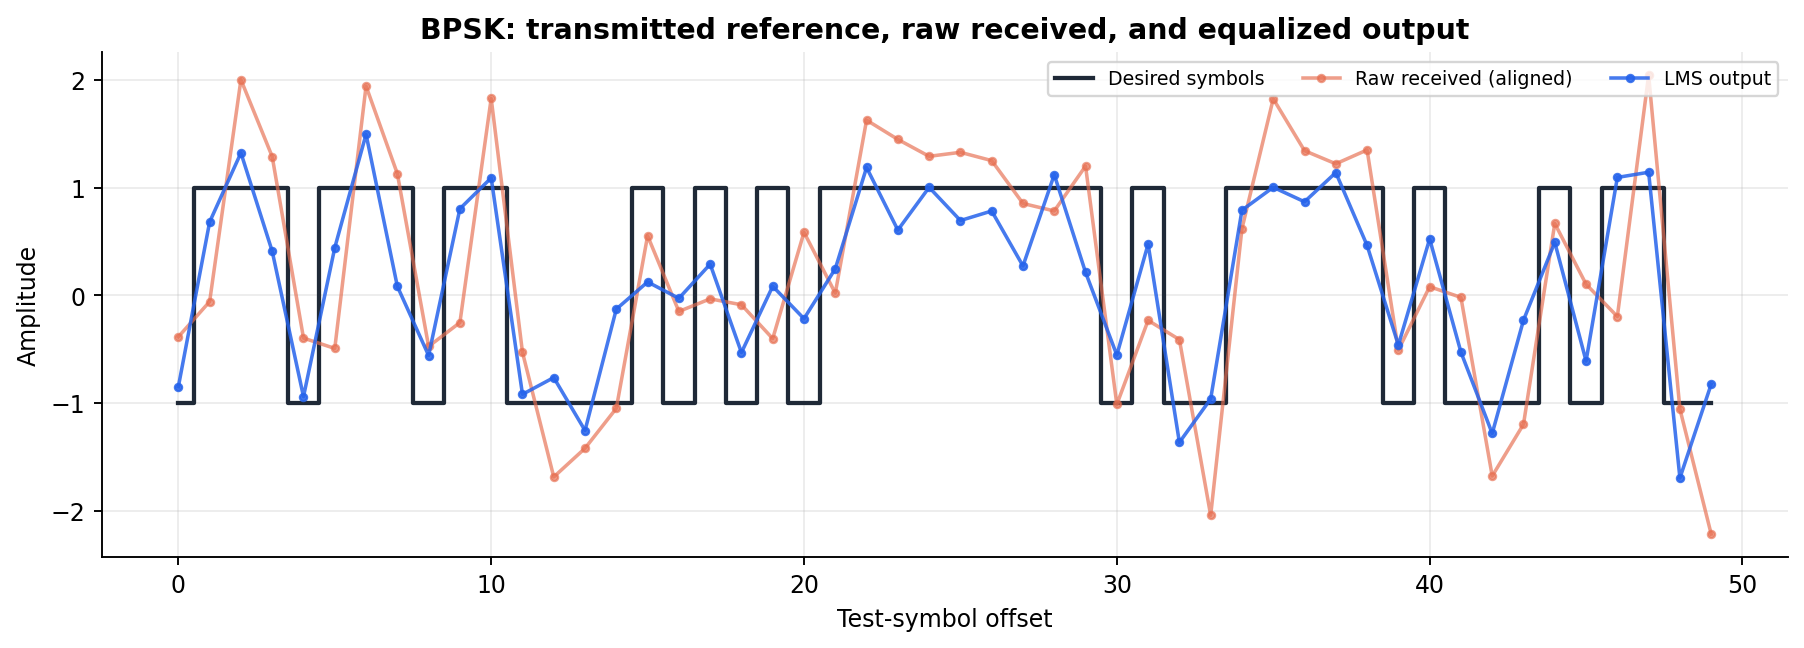
\includegraphics[width=\linewidth]{03_bpsk_waveforms.png}
\centering{\tiny Example BPSK signal sequence}
\end{columns}
\end{frame}

\begin{frame}{3. Informal picture: complete simulator}
\centering
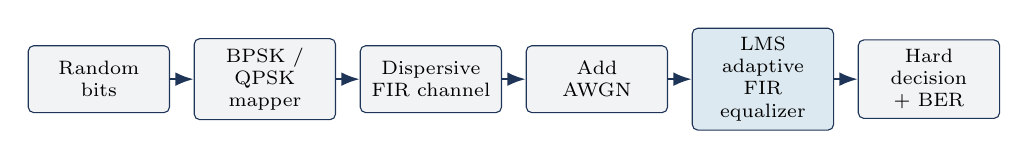
\begin{tikzpicture}[
  node distance=0.30cm,
  box/.style={draw=navy,rounded corners=2pt,fill=navy!6,minimum width=1.67cm,
  minimum height=0.85cm,text width=1.56cm,align=center,font=\scriptsize},
  >=Latex]
  \node[box] (bits) {Random\\ bits};
  \node[box,right=of bits] (map) {BPSK / QPSK\\ mapper};
  \node[box,right=of map] (chan) {Dispersive\\ FIR channel};
  \node[box,right=of chan] (noise) {Add\\ AWGN};
  \node[box,right=of noise,fill=accent!15] (lms) {LMS adaptive\\ FIR equalizer};
  \node[box,right=of lms] (dec) {Hard decision\\ + BER};
  \foreach \a/\b in {bits/map,map/chan,chan/noise,noise/lms,lms/dec}
    \draw[->,thick,navy] (\a)--(\b);
\end{tikzpicture}
\vspace{0.65cm}
\begin{block}{Training path versus evaluation path}
Known transmitted symbols provide an error signal \textbf{only during training}. After $2500$ time samples, weights are frozen; $9000$ subsequent reference symbols are used only for error counting.
\end{block}
\medskip
\centering{\small \textbf{One algorithm, two signal alphabets, multiple parameter sweeps.}}
\end{frame}

\begin{frame}{4. Informal picture: what LMS learns}
\begin{enumerate}\setlength{\itemsep}{10pt}
\item Start with zero equalizer taps.
\item Form a weighted sum of the latest received samples.
\item Compare this output with a \textbf{known, delay-aligned training symbol}.
\item Update the taps using an error-scaled input vector.
\item Freeze taps and measure BER on unseen symbols.
\end{enumerate}
\vspace{0.3cm}
\begin{block}{Intuition}
LMS learns to undo some of the spreading caused by the channel, while trading off residual ISI and noise enhancement.
\end{block}
\end{frame}

\begin{frame}{5. Mathematical model: channel and FIR equalizer}
\begin{align*}
 \textbf{Channel:}\quad r[n] &= \sum_{\ell=0}^{L_h-1} h[\ell]s[n-\ell] + v[n]\\[8pt]
 \textbf{Tap input:}\quad \mathbf{x}[n] &= [r[n],r[n-1],\ldots,r[n-M+1]]^T\\[8pt]
 \textbf{Output:}\quad y[n] &= \mathbf{w}^H[n]\mathbf{x}[n]\\[8pt]
 \textbf{Reference:}\quad d[n] &= s[n-D]\\[8pt]
 \textbf{Error:}\quad e[n] &= d[n]-y[n]
\end{align*}
\vspace{0.2cm}
\centering{\small $M=9$ taps and decision delay $D=2$ in baseline experiments.}
\end{frame}

\begin{frame}{6. Mathematical model: Wiener objective}
\begin{block}{Minimize mean-square error}
\[J(\mathbf w)=E[|d-\mathbf w^H\mathbf x|^2]\]
\end{block}
\begin{align*}
 \mathbf R &= E[\mathbf x\mathbf x^H],\qquad \mathbf p=E[\mathbf x d^*]\\[6pt]
 \frac{\partial J}{\partial \mathbf w^*} &= \mathbf R\mathbf w-\mathbf p\\[6pt]
 \mathbf R\mathbf w_{\rm opt} &= \mathbf p \quad\Rightarrow\quad
 \mathbf w_{\rm opt}=\mathbf R^{-1}\mathbf p
\end{align*}
\vspace{-0.14cm}
\begin{alertblock}{Why LMS instead of solving the matrix equation?}
LMS replaces expected gradients with single-sample estimates: it does not require explicitly estimating or inverting $\mathbf R$.
\end{alertblock}
\end{frame}

\begin{frame}{7. Mathematical model: complex-correct LMS update}
\begin{block}{Core recursion}
\[\boxed{\mathbf w[n+1]=\mathbf w[n]+\mu\,\mathbf x[n]e^*[n]}\]
\end{block}
\vspace{0.1cm}
\begin{itemize}\setlength{\itemsep}{7pt}
\item $\mu$: step size; controls convergence speed and fluctuations.
\item Complex conjugation $e^*[n]$ is needed for \textbf{QPSK}.
\item With $y=\mathbf w^H\mathbf x$, use NumPy \texttt{np.vdot(w, x)}.
\item Mean-convergence guidance: $0<\mu<2/\lambda_{\max}(\mathbf R)$ under idealized assumptions; not a blanket stability guarantee.
\end{itemize}
\vspace{0.2cm}
\centering{\small Training and test data are separated before BER evaluation.}
\end{frame}

\begin{frame}{8. Results: convergence and QPSK constellation}
\begin{columns}[T]
\column{.50\textwidth}
\centering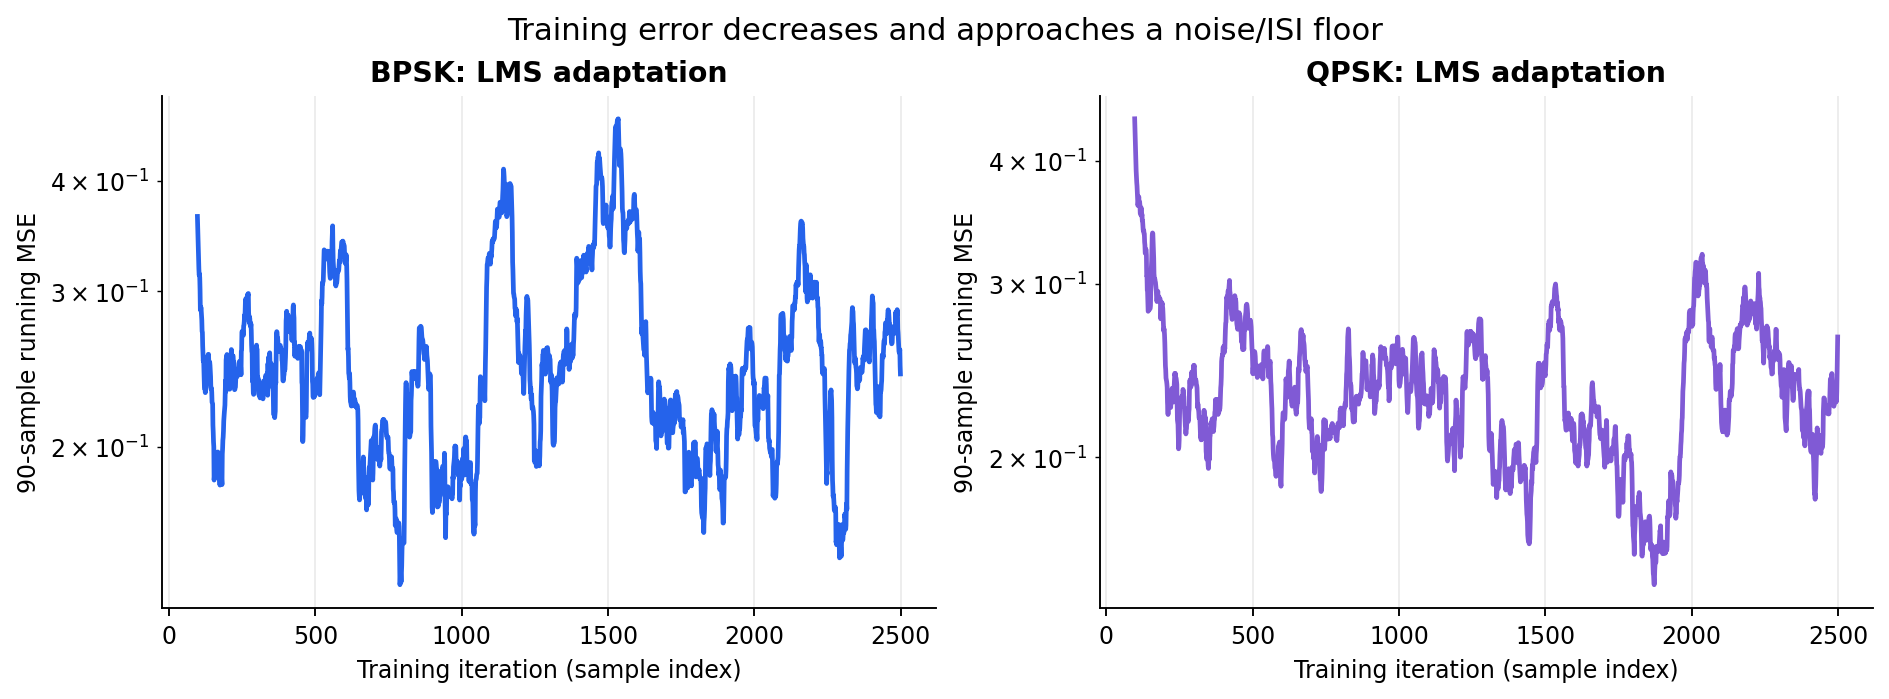
\includegraphics[width=\linewidth]{01_mse_convergence.png}\\
{\scriptsize Training MSE approaches a floor.}
\column{.50\textwidth}
\centering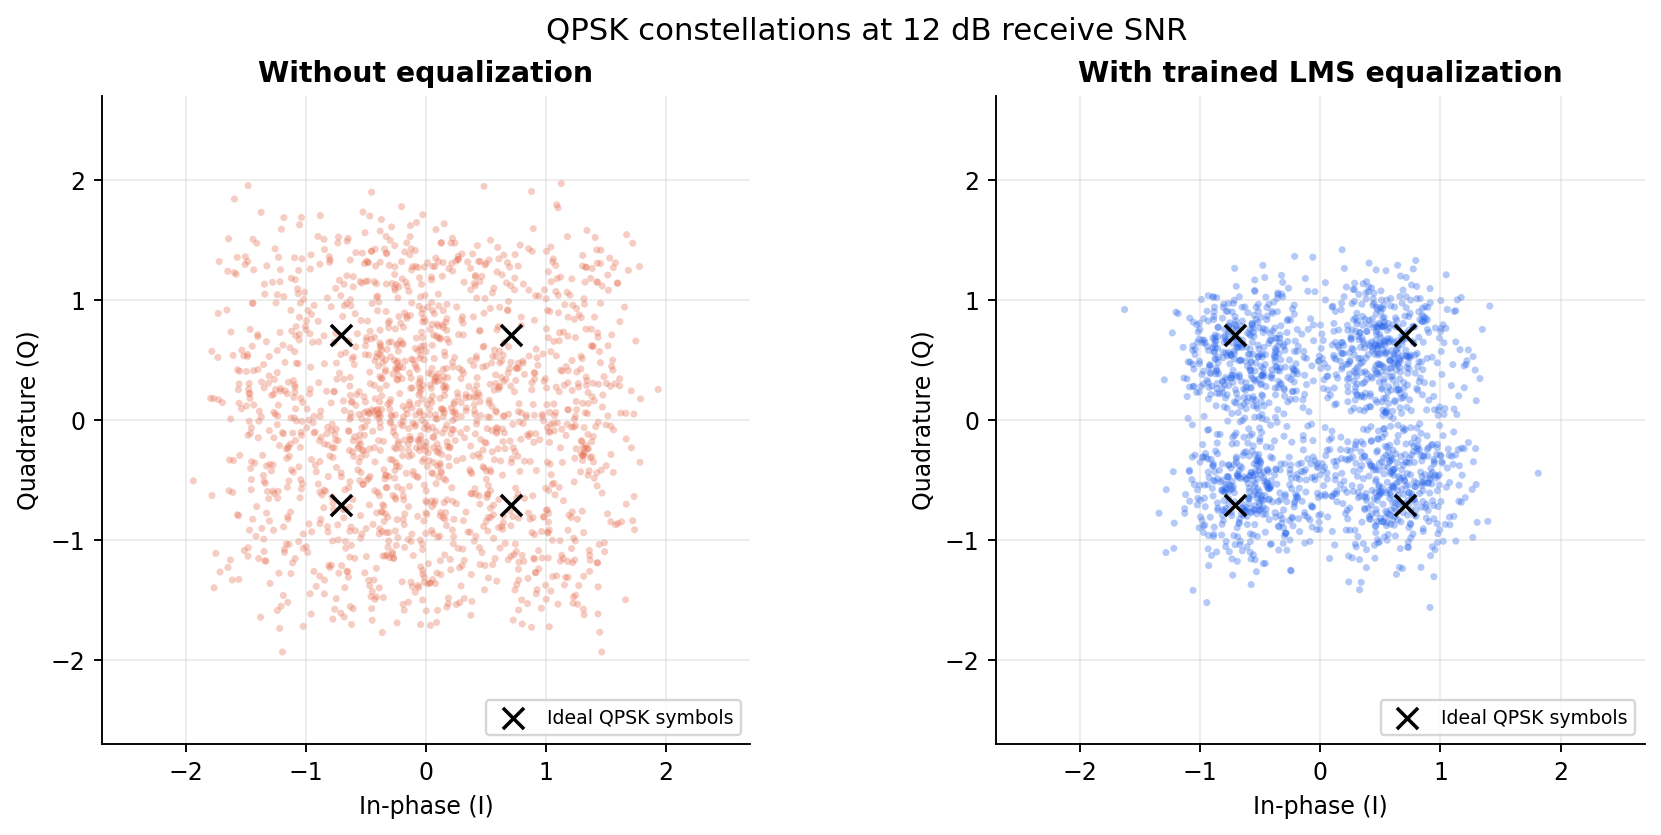
\includegraphics[width=\linewidth]{02_qpsk_constellation.png}\\
{\scriptsize QPSK points become better clustered.}
\end{columns}
\vspace{0.30cm}
\centering{\footnotesize Main setting: SNR 12 dB, $M=9$, $\mu=0.018$, channel $[0.90,\,0.65,\,-0.35]$.}
\end{frame}

\begin{frame}{9. Results: measured BER versus SNR}
\begin{columns}[T]
\column{.62\textwidth}
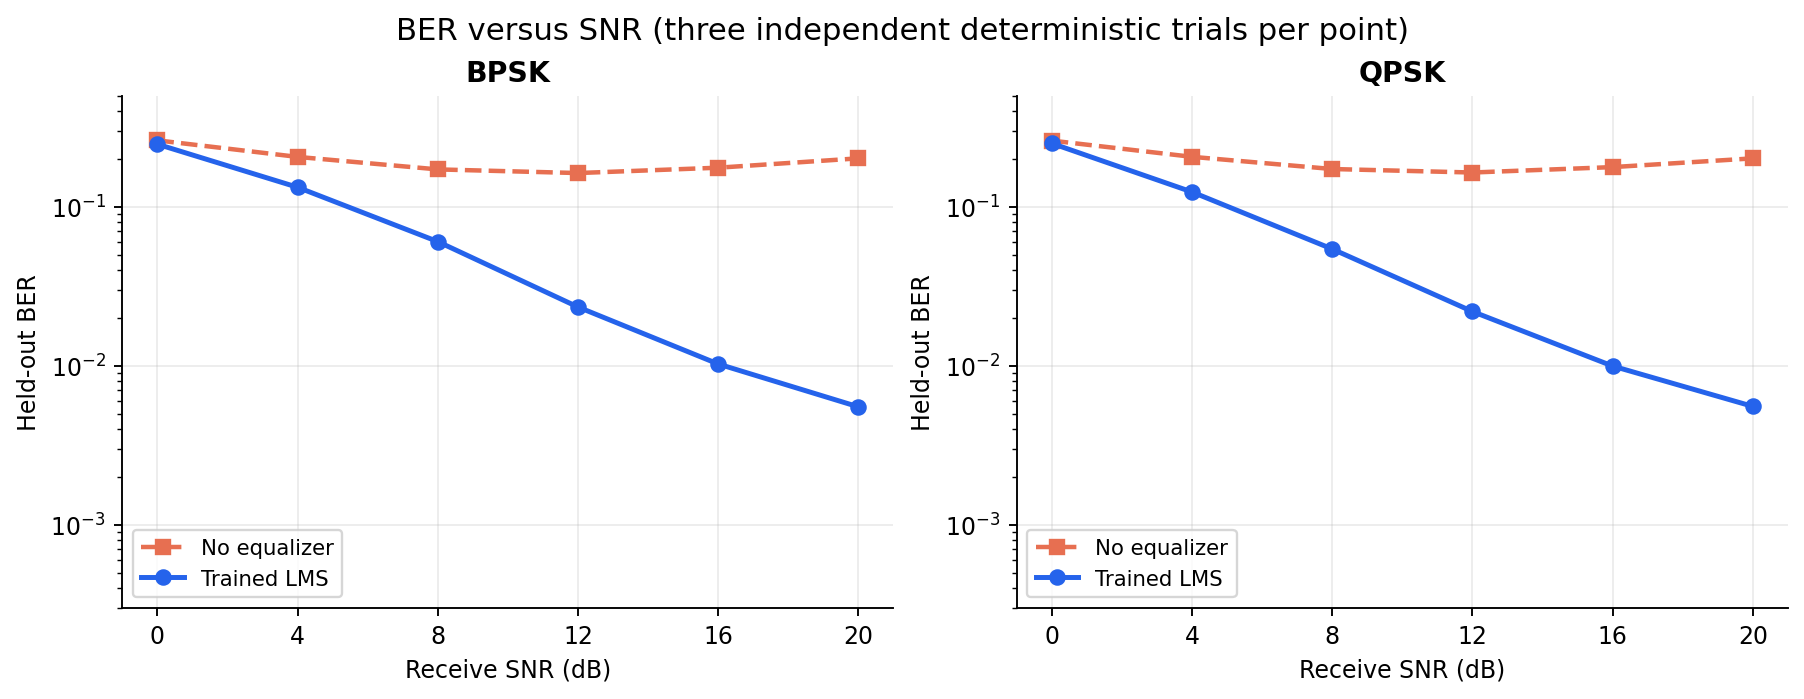
\includegraphics[width=\linewidth]{06_ber_vs_snr.png}
\column{.36\textwidth}
\textbf{At 12 dB, seed 2026}\vspace{0.2cm}
\begin{tabular}{@{}lrr@{}}\toprule
& Raw & LMS \\ \midrule
BPSK & .1549 & .0217 \\
QPSK & .1591 & .0247 \\ \bottomrule
\end{tabular}
\vspace{0.4cm}
{\scriptsize BER graph: mean of three seeded trials per SNR. Raw ISI channel can show a nonmonotonic BER floor.}
\end{columns}
\end{frame}

\begin{frame}{10. Results: step size and filter length}
\begin{columns}[T]
\column{.50\textwidth}
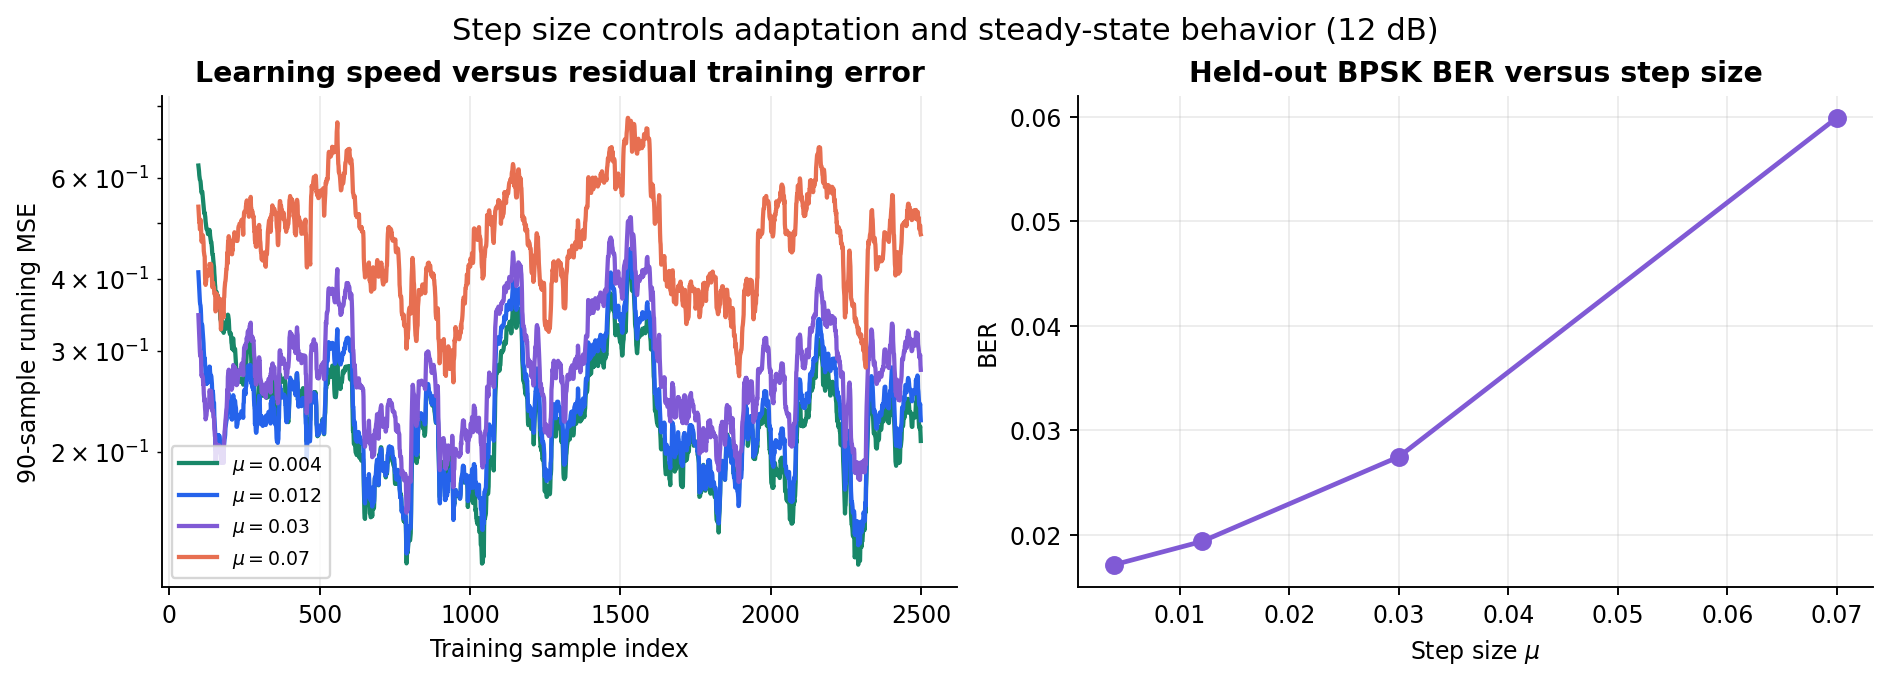
\includegraphics[width=\linewidth]{04_stepsize_sweep.png}
\column{.50\textwidth}
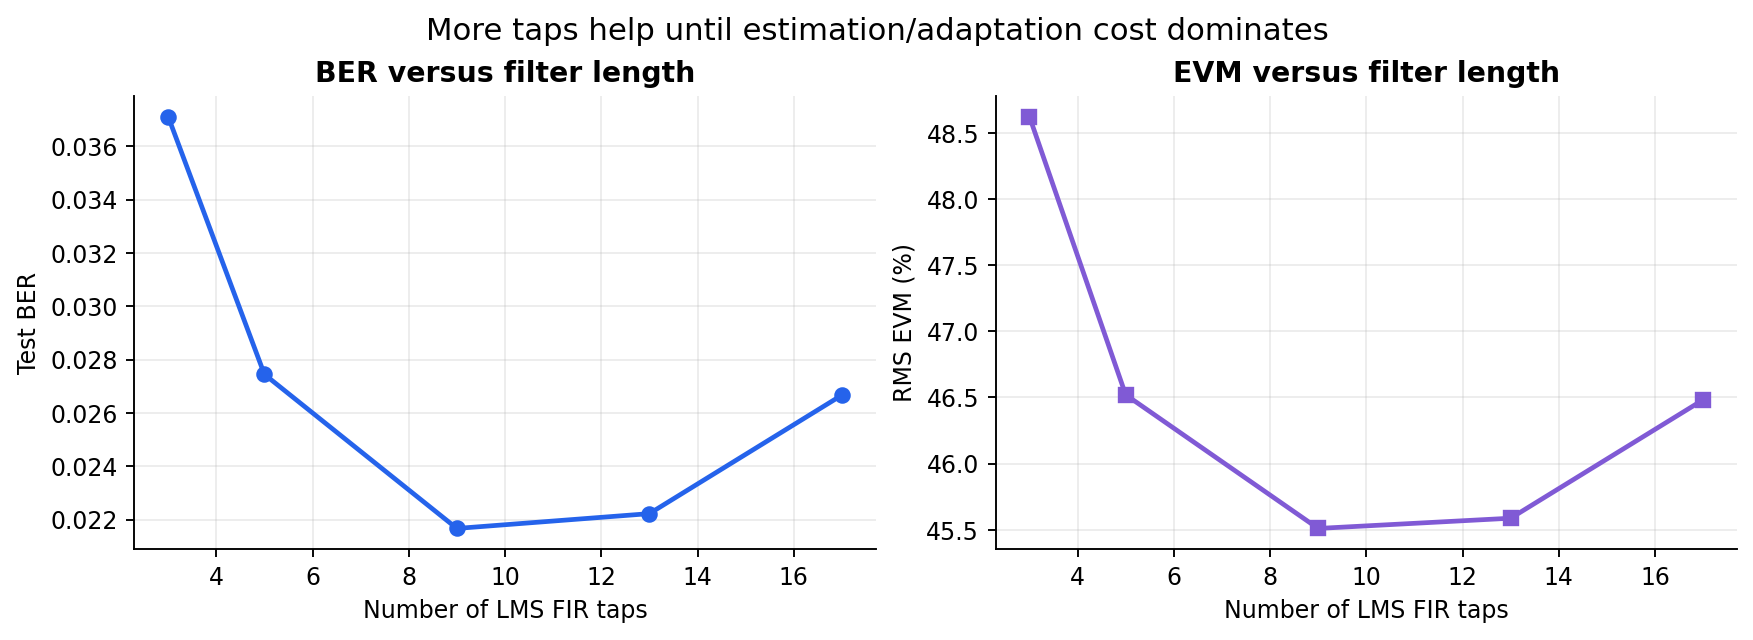
\includegraphics[width=\linewidth]{05_filter_length_sweep.png}
\end{columns}
\vspace{0.28cm}
\begin{block}{Main conclusions / limitations}
\footnotesize Smaller or larger $\mu$ and more taps are not automatically better. Results are for a known preamble, stationary channel, coherent symbols and symbol-rate samples; no live-radio, pulse shaping, or timing recovery is claimed.
\end{block}
\vspace{-0.05cm}
\centering{\scriptsize Files: \texttt{LMS\_Equalizer.ipynb}, \texttt{lms\_equalizer.py}, \texttt{experiments.py}; technical report and sources included.}
\end{frame}

\end{document}
